\documentclass[]{report}
\usepackage{minted}
\usepackage[utf8]{inputenc}
\usepackage{amssymb}
\usepackage{amsmath}
\usepackage{booktabs}
\usepackage{graphicx}
\graphicspath{{images/}}
\usepackage{caption}
\usepackage{subcaption}
\usepackage{braket}
\usepackage{changepage}
\usepackage[a4paper,width=150mm,top=0.75in,bottom=0.75in]{geometry}
\usepackage{mwe}
\usepackage{float}
\usepackage[font=footnotesize,labelfont=bf]{caption}
\usepackage{bbold}
\usepackage{framed}
\usepackage{sidecap}
\usepackage{hyperref}
\usepackage{setspace}
\usepackage{notoccite}
\usepackage{cleveref}
\usepackage{physics}
\usepackage{siunitx}
\usepackage[style=ieee, citestyle=numeric-comp, backend=biber]{biblatex}

\setlength{\parindent}{0pt}
\renewcommand{\figurename}{Fig.}
\newtheorem{theorem}{Theorem}

\title{Towards Accurate DeepMD Potentials for Aqueous Interfaces}
\author{Christian Loer Llemit\\[1cm]{Supervisors:}\\{\small  Ali
Hassanali}\\{\small Cesare Malosso}\\{\small Edward Donkor} }
\date{August 2024}

\addbibresource{references.bib}

\begin{document}

\maketitle
\pagenumbering{arabic}

\chapter*{Acknowledgement}
\addcontentsline{toc}{chapter}{Acknowledgement}




I would like to thank my supervisor, Dr. Ali Hassanali, for all the guidance that made the completion of this thesis possible. I am grateful to him for dedicating his valuable time to providing constructive criticism and for instilling in me the importance of always asking questions and exploring all possible solutions to unresolved problems. I would also like to thank my co-supervisor, Cesare Malosso, for guiding me in preparing codes, for orienting me on how the code works, and for his feedback. My thanks also go to my co-supervisor, Edward Donkor, for sharing some of his codes and for his feedback.

I would like to express my gratitude to the atomistic simulations group for criticizing my presentation, which greatly helped me improve. I am thankful to all the professors for dedicating their time and sharing their expertise with future scientists. I also extend my thanks to the library staff for their assistance and to my fellow classmates for the fruitful discussions.

I would like to thank Alexandra Santos-Putungan and Darwin Putungan for encouraging me to apply for the postgraduate diploma program. I am deeply grateful to my family for their unwavering support throughout my journey.

Lastly, I extend my gratitude to ICTP for being a wonderful institution that helps students from developing countries.

\tableofcontents

\setstretch{1.5}

\chapter*{Abstract}
\addcontentsline{toc}{chapter}{Abstract}

This thesis explores the challenges and issues in modelling the many-body potential energy surface
for liquid water interfaces by means of developing deep neural network potential  scheme for molecular dynamics simulations (DPMD), as implemented in DeePMD-kit. We focus on modelling  neat water interfaces by training the datasets of bulk and bulk+interface systems with Density Functional Theory (DFT) level of accuracy and linear scale efficiency of empirical force fields. In addition, DPMD can be parallelized due to its local decomposition and  near-neighbor dependence of  atomic energies. The generated deep neural network potential (NNP) was assessed according to its predictability in obtaining relevant system properties such as mass density, surface tension, and dipole orientation. Due to numerical instabilities using SCAN functional for interfaces, we used instead a similar  but accurate and numerically efficient regularized-restored r$^2$SCAN functional in labelling the datasets. Neural network potential trained on only bulk
systems did not perform well when used on trajectories containing interfaces. Adding interface dataset to the training
did improve the prediction  of macroscopic properties, implying that surface defects
play a role in surface properties of water. In addition, the bulk+interface trained NNP have the same accuracy as the reference NNP used but with a smaller  training dataset. All the models  fail to describe microscopic properties such as dipole orientation at the surface but still obtain good macroscopic properties such as surface tension for the bulk+interface trained NNP.  Finite size effects  and  long-range electrostatic interactions might play a role in obtaining  discrepancies at the microscopic level.

\chapter{Introduction}

\section{Objectives}

Describe importance of analyzing interfaces. Surface tension of different
solutes.

\begin{itemize}
    \item To develop accurate and transferrable DeepNN potentials for
          interfaces
    \item To explore the quality of the training data set in improving the
          description of water interfaces.
    \item To understand reliability of the current architecture of DeepMD in
          dealing with interfaces.

\end{itemize}
\chapter{Theory}

Interactomic Potential Energy Surface (PES) is an important property of the
system
that enables us to explain and predict materials properties such as interfacial
energies, thermal expansion, cohesion, surface tension as well as chemical
reactions.
Representing PES accurately and efficiently is a major goal in molecular
modelling.
Existing approaches to PES modelling includes ab-initio models based on DFT,
empirical force fields fitted with experimental data, and the
relatively recent
machine learning based approach. The first one is accurate, parameter-free, and
transferable but has bad scaling with system size. The second one is
computationally efficient but has limited accuracy and transferability.
The third one combines both the advantages of the two previous approaches in
that it efficiently represents the PES for a
wide variety of systems with the level of accuracy of ab initio quantum
mechanics
models and scales for large systems.

% https://en.wikipedia.org/wiki/Interatomic_potential
This work will focus on a particular scheme for molecular modelling, the deep
neural network
potential molecular dynamics.

\section{Basics of Machine Learning}
Before dealing with deep potential molecular dynamics, one must have a basic
understanding on the principles of machine learning. Machine Learning (ML)
falls
under
the umbrella
term of Artificial Intelligence
(AI)
that focuses on developing algorithms that enable computers to learn from and
make decisions based on data. It is based on the idea that systems can
automatically improve their performance on a task through experience without
human intervention. The algorithm will understand the data by deconstructing it
in terms of hierarchy of concepts, with each concept defined through its
relation to simpler concepts. This allows the algorithm to learn complicated
concepts by building from simpler ones. Tasks such as classification,
regression, transcription, clustering, translation, to name a few can be solved
by ML.

% https://www.deeplearningbook.org/contents/intro.html
% https://www.deeplearningbook.org/contents/ml.html

Regression learning works by allowing the program to fit an input of dimension
$\mathfrak{R}^n$ to an output of lower dimension $\mathfrak{R}^m$ by applying a
mapping function $f$.
Regression learning is an example of supervised learning since it
involves training a model on a labeled dataset. In practice, the labeled data
set is split into two: the training/learning and the testing/validation
data. The first one is feed to the algorithm while the second one is used to
validate the accuracy of the prediction.

Deep Learning is a type of ML that mimics the function of a
neuron in the living systems. It is divided into layers that constitutes the
input, output and multiple hidden layers where each layers contains collection
of
`neurons' or nodes as schematically shown in Figure \ref{fig:DL}. An algorithm
with one
hidden layer is
considered an Artificial Neural Network (ANN). Specifically, the algorithm is a
subset of Regression learning that maps an input to an output. Deep forwarded
network, also called
feed-forward neural network, refers to the idea that information moves in only
one direction from input, through the hidden layers,  to the output.  The goal
of a feedforward network is to approximate the mapping $y = f(x; w)$ of input
vector $x$ to an output vector $y$ by optimizing the values of the
parameters/weights $w$. Networking works by applying composition of many
different
functions. For a network with  $N$ layers depth, $N$ functions $f^1, f^2,
    \cdots, f^N$ will be
chained in succession to form $f(x) = f^N(\cdots f^2(f^1(x)))$. The innermost
function
refers to the first layer while the outermost function refers to the output
layer. Those functions that are in between refer to hidden layers since their
outputs are not desired.

% change graph 
% https://www.bmc.com/blogs/deep-neural-network/
\begin{figure}[h!]
    \centering
    \includegraphics[width=0.5\linewidth]{images/DL.png}
    \caption{Typical configuration of a Deep Learning algorithm with 2 hidden
        layers that maps a $\mathfrak{R}^3$ input vector to a scalar output
        vector.}
    \label{fig:DL}
\end{figure}

To explain how each functions work, we look closely to the mathematical
interpretation of a neuron, as schematically shown in
Figure~\ref{fig:neuron_struc}. For a given artificial neuron $j$, let there be
$n+1$ inputs with signals $x_0$ through $x_n$ and weights $w_{0j}$ through
$w_{nj}$. The $x_0$ input is assigned the value +1, which makes it a bias input
with $w_{0j}$ = $b_j$. There will be $n$ actual inputs to the neuron: from
$x_1$ to $x_n$. The inputs will be weighted sum and the result is used as an
argument of the threshold function or activation function $\varphi$. Once the
function reaches a threshold value $\theta_j$ or more, it will give the output
or activation $a_j$ of the  $j$th neuron. Mathematically,

\begin{equation} \label{eq:activation_funct}
    a_j =   \varphi \left(\sum_{i=0}^{n} w_{ij}^T x_i \right) =  \varphi
    \left( z_{j}\right)
\end{equation}

Typical activation functions are Heaviside function, sigmoid, and rectified
linear functions (ReLu).

\begin{figure}[h!]
    \centering
    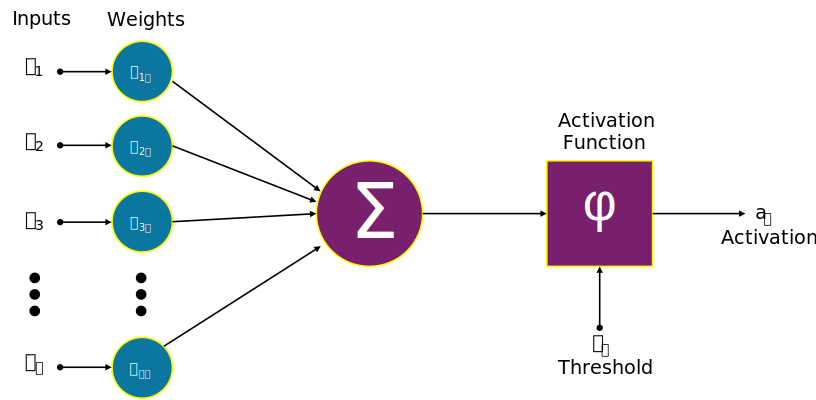
\includegraphics[width=0.5\linewidth]{images/artificial_neuron.pdf}
    \caption{The mathematical model of a neuron as first introduced by
        McCulloch and Pitts \cite{mcculloch1943logical}. Image taken at
        commons.wikimedia.org/wiki/File:Artificial\_neuron\_structure.svg}
    \label{fig:neuron_struc}
\end{figure}

One way to assess the performance of the training model is to compute the loss
function, or cost function, $\mathcal{L}$ with respect to the weights. A simple
choice is to compute the mean squared error
(MSE)
between the predicted $\hat{y}^{(\text{test})}$ and actual $y^{(\text{test})}$
value within the testing
dataset.

\begin{equation}
    \mathcal{L}^{(\text{test})}(w) = MSE^{(\text{test})} = \frac{1}{M} \sum_i^M
    \left(
    \hat{y}_i^{(\text{test})} -
    y_i^{(\text{test})} \right)^2  = \frac{1}{M} \sum_i^M
    \mathcal{L}^{(\text{test})}_i
\end{equation}

where $M$ is the number of test examples in the dataset. An algorithm should be
introduced to minimize the error  while allowing to gain
experience by incorporating a training dataset.
An intuitive way is to minimize the MSE on the training dataset with respect to
the weights by carrying out
the minimization problem called Gradient Descent

\begin{equation}
    \nabla_w \text{MSE}_\text{train} \approx 0
\end{equation}

The weights are updated by subtracting a factor proportional to the
gradient of the loss function.

\begin{equation}
    w_{n+1} = w_n - \epsilon  \grad_w \mathcal{L}(w)
\end{equation}

where $\epsilon$ is the learning rate and $n$ is the iteration step. Stochastic
Gradient Descent extends the well-known Gradient Descent algorithm. Instead of
computing the
actual gradient, which is computationally expensive for large training
datasets,  it is replaced
by an approximate gradient of a random subset of the training data. The loss
function is minimized by taking  the average gradient with respect to the
weights for $M'$ random minibatches of examples from the training set

\begin{align}
    \grad_w \mathcal{L}(w) \approx \frac{1}{M'} \sum_{i=1}^{M'} \grad_w L_i
\end{align}
where $L_i$ is the loss function of a specific training example $i$.

The stochastic gradient descent does a good job in reducing the computational
time, but the learning process can still be improved by implementing the
backpropagation algorithm. The algorithm works by computing the gradient of
the loss function with respect to each weights by utilizing chain rules in
backward fashion, from last layer to the first.

Without going to full derivation, the idea is to measure the sensitivity of the
loss function  to variations in  parameters such as weights,
biases and the activations.  For simplicity, consider the case of $N$ layers
with one neuron each. For one training example,  the loss function will be
$\mathcal{L}_0 = \left(a^{(N)} - y \right)^2$ where $a^{(N)}$ is the activation
of the
neuron at the last layer $N$ and $y$ is the actual value of the training
example. From eqtn.~\eqref{eq:activation_funct}, the activation will depend on
the previous layer

\begin{align}
    a^{(N)} & = \varphi \left( w^{(N)} a^{(N-1)} + b^{(N)} \right)
    \Longrightarrow
    \varphi
    \left( z^{(N)} \right)
\end{align}

where $w^{(N)}$ and $b^{(N)}$ are the weights and biases of the $N$th layer.
Taking relevant partial derivatives

\begin{align}
    \pdv{z^{(N)}}{w^{(N)}}       & = a^{(N-1)}, \quad \pdv{z^{(N)}}{b^{(N)}}
    =1,
    \quad \pdv{z^{(N)}}{a^{(N-1)}} = w^{(N)}                                 \\
    \pdv{a^{(N)}}{z^{(N)}}       & = \varphi'
    \left( z^{(N)} \right)                                                   \\
    \pdv{\mathcal{L}_0}{a^{(N)}} & = 2 \left(a^{(N)} - y \right)
\end{align}

By Chain Rule,

\begin{align}
    \pdv{\mathcal{L}_0}{w^{(N)}}		      =
    \pdv{\mathcal{L}_0}{a^{(N)}}
    \pdv{a^{(N)}}{z^{(N)}} \pdv{z^{(N)}}{w^{(N)}}    & = 2 \left(a^{(N)} - y
    \right)
    \varphi'
    \left( z^{(N)} \right)  a^{(N-1)}
    \\
    \pdv{\mathcal{L}_0}{a^{(N-1)}}		      =
    \pdv{\mathcal{L}_0}{a^{(N)}}
    \pdv{a^{(N)}}{z^{(N)}} \pdv{z^{(N)}}{a^{(N-1)} } & = 2 \left(a^{(N)} - y
    \right)
    \varphi'
    \left( z^{(N)} \right)  w^{(N)}
    \\
    \pdv{\mathcal{L}_0}{b^{(N)}}		      =
    \pdv{\mathcal{L}_0}{a^{(N)}}
    \pdv{a^{(N)}}{z^{(N)}} \pdv{z^{(N)}}{b^{(N)}}    & = 2 \left(a^{(N)} - y
    \right)
    \varphi'
    \left( z^{(N)} \right)
\end{align}

To generalize to more than one neurons per layer, one must introduce subscript
so that $a^{(N)}_j$ denotes the activation of  $j$th neuron in the $N$th layer
while $w^{(N)}_{jk}$ is the weight that connects the $j$th neuron in the $N$th
layer with the $k$th neuron in the previous layer. Also, define $z^{(N)}_j =
    \sum_k
    w^{(N)}_{jk} a^{(N-1)}_k + b^{(N)}_j$. The chain rule is modified as
follows

\begin{align}
    \pdv{\mathcal{L}_0}{w^{(N)}_{jk}} & =
    \pdv{\mathcal{L}_0}{a^{(N)}_j}
    \pdv{a^{(N)}_j}{z^{(N)}_j} \pdv{z^{(N)}_j}{w^{(N)}_{jk}}  =
    \pdv{\mathcal{L}_0}{a^{(N)}_j}
    \varphi'
    \left( z^{(N)}_j \right)  a^{(N-1)}_k
    \label{eq:back_prop1}
    \\
    \pdv{\mathcal{L}_0}{a^{(N-1)}_k}  & = \sum_{j=0}^{n_N-1}
    \pdv{\mathcal{L}_0}{a^{(N)}_j}
    \pdv{a^{(N)}_j}{z^{(N)}_j} \pdv{z^{(N)}_j}{a^{(N-1)}_k }  =
    \sum_{j=0}^{n_N-1} \pdv{\mathcal{L}_0}{a^{(N)}_j}
    \varphi'
    \left( z^{(N)}_j \right)  w^{(N)}_{jk}
    \label{eq:back_prop2}
    \\
    \pdv{\mathcal{L}_0}{b^{(N)}_j}    & =
    \pdv{\mathcal{L}_0}{a^{(N)}_j}
    \pdv{a^{(N)}_j}{z^{(N)}_j} \pdv{z^{(N)}_j}{b^{(N)}_j}     =
    \pdv{\mathcal{L}_0}{a^{(N)}_j}
    \varphi'
    \left( z^{(N)}_j \right)
\end{align}

Eqtn.~\eqref{eq:back_prop1} can be rewritten by using
eqtn.~\eqref{eq:back_prop2} for arbitrary layer $l$ as

\begin{equation}
    \pdv{\mathcal{L}_0}{w^{(l)}_{jk}} =  a^{(l-1)}_k \varphi'\left( z^{(l)}_j
    \right) \sum_{j=0}^{n_{l+1}-1}
    w^{(l+1)}_{jk} \varphi'
    \left( z^{(l+1)}_j \right)	 \pdv{\mathcal{L}_0}{a^{(l+1)}_j}
\end{equation}

This equation is what called the backpropagation formula where it got its name
since the error
of the
previous layer depends on the values of the forward layers. This formula
estimates the gradient that goes into updating the weights.

% rephrase
Deep learning continues to evolve rapidly, driven by advances in
computational power, availability of large datasets, and innovative algorithms.
It holds the promise of transforming various aspects of human life and industry
by enabling more intelligent, autonomous systems.

\section{Deep Neural Molecular Dynamics}
Machine Learning potentials have very flexible functional form that allows to
represent reference data of quantum-mechanics accuracy at a cost that is
comparable to empirical force fields. Particularly, deep learning molecular
dynamics relies on using deep neural network trained potential (DeepPotential)
to simulate the
dynamics of the molecular system.  DeepPotential Method have basic assumptions
\cite{zhang2018deep,zhang2018end},
namely

\begin{itemize}

    \item  Potential energy surface (PES) is extensive, it can be expressed as
          sum		of	     short-ranged many body atomic
          contributions
          \begin{equation}
              \Phi(\vec{r}_1,\vec{r}_1,\hdots, \vec{r}_N) = \sum_i
              \Phi_i(\{\mathcal{R}^i\})
          \end{equation}
          where $\Phi_i$ is represented by	     a		 function
          of atomic coordinates within the local environment of      the
          $i$th atom.
    \item  the function $\Phi_i$ continuous and differentiable
          of atomic coordinates,
    \item the function $\Phi_i$ preserves the translational, rotational,
          and
          permutational symmetry of the system,
    \item the function $\Phi_i$ is represented from end-to-end by a deep
          neural network trained on DFT data
\end{itemize}

In regard to the first assumption, one can define first a global coordinate
matrix

\begin{equation}
    \mathcal{R} =  \mqty( x_1 & y_1 & z_1 \\ x_2 & y_2 & z_2 \\ \vdots & \ddots
    &
    \vdots \\
    x_N & y_N & z_N)
\end{equation}

that lists the absolute coordinates of all the atoms. Then, define a relative
coordinate matrix of the local environment centered on atom  $i$ as

\begin{equation}
    \mathcal{R}^i =  \mqty( x_{1i} & y_{1i} & z_{1i} \\ x_{2i} & y_{2i} &
    z_{2i}
    \\ \vdots & \ddots
    &
    \vdots \\
    x_{N_i i} & y_{N_i i} & z_{N_i i})
\end{equation}

where $N_i$ are the number of atoms within the cutoff radius $r_c$ from the
central $i$th atom. Note that the coordinates are measured with respect to this
central atom, $\vec{r}_{ji} = \vec{r}_{j}- \vec{r}_{i}$. To impose smoothness
of the function, the relative coordinate matrix is mapped to  a renormalized
coordinate matrix

\begin{equation}
    \tilde{\mathcal{R}^i} =  \mqty( s(r_{1i}) &
    \frac{s(r_{1i}) x_{1i}}{r_{1i}}
    &	 \frac{s(r_{1i}) y_{1i}}{r_{1i}} &
    \frac{s(r_{1i}) z_{1i}}{r_{1i}} \\
    s(r_{2i}) &
    \frac{s(r_{2i}) x_{2i}}{r_{2i}}
    &	 \frac{s(r_{2i}) y_{2i}}{r_{2i}} &
    \frac{s(r_{2i}) z_{2i}}{r_{2i}}
    \\ \vdots & \vdots & \vdots
    &
    \vdots \\
    s(r_{N_i i}) &
    \frac{s(r_{N_i i}) x_{N_i i}}{r_{N_i i}}
    &	 \frac{s(r_{N_i i}) y_{N_i i}}{r_{N_i i}} &
    \frac{s(r_{N_i i}) z_{N_i i}}{r_{N_i i}} )
\end{equation}

where $s(r)$ is a smooth switching function defined as

\begin{equation}
    s(r) = \begin{cases}
        \frac{1}{r}                                   & , r   < r_s        \\
        \frac{1}{r} \left[x^3 (-6x^2+15x-10)+1\right] & , r_s \leq r < r_c \\
        0                                             & , r   \geq r_c
    \end{cases}
\end{equation}

where $x = \frac{r- r_s}{r_c-r_s}$, $r_c$ is the cutoff radius and $r_s$ is the
distance from atom $i$ where smoothing is applied. The	smooth cut-off
parameter $r_s$ allows the components of $\tilde{\mathcal{R}^i}$ to
go to zero smoothly at the boundary of the local region defined by $r_c$.
Particularly, the smoothing function $s(r)$ reduces the weight of atoms that
are farther from atom $i$, and at the same time removing the discontinuity
introduced by the cut-off. The renormalized coordinate matrix will serve as a
local descriptor that will feed into a specific deep neural network
NN$^{\alpha_i}$ where $\alpha_i$ is the chemical type of atom $i$. The output
of the neural network is the local atomic energy $\epsilon_i$ of the $i$th
atom. Then, the PES is given by the sum of the local atomic energies

\begin{equation}
    E = \sum_i^N	\epsilon_i
\end{equation}

while the atomic forces are

\begin{equation}
    \vec{F}_i = - \nabla_{\vec{R}_i} E = - \sum_i^N \nabla_{\vec{R}_i}
    \epsilon_i
\end{equation}

and the components of stress tensor is defined as

\begin{equation}
    \Xi_{\alpha \beta} = \sum_i^N R_{i\alpha} F_{i\beta}
\end{equation}

The training is performed with the stochastic descent method, minimizing the
loss function with respect to the weights of the deep neural network. The
evaluation of the gradient is carried out using backpropagation algorithm,
with the loss function defined as

\begin{equation}
    \mathcal{L} =   \frac{1}{M} \sum_l^M  \left[  p_E \left(\hat{E}^l- E^l
        \right)^2 +
        p_F \abs{\hat{\vec{F}}^l- \vec{F}^l}^2 + p_V \left(\hat{\Xi}^l- \Xi^l
        \right)^2 \right]
\end{equation}

where $M$ is the number of examples in the minibatch; $\hat{E}^l$,
$\hat{\vec{F}}^l$, and $\hat{\Xi}^l$
are the predicted energies, total forces, and stress tensor; $E^l$,
$\vec{F}^l$, and $\Xi^l$ are
the DFT
energies, forces, and stress tensor; $p_E$, $p_F$, and $p_V$  are tunable
prefactors
useful to improve the
efficiency of the training.
\chapter{Methodology}
Initial trajectories were generated using Molecular Dynamics implemented in LAMMPS \cite{LAMMPS}. The pair potential used is based on the previously trained deep neural network potential (NNP) conducted by Sanchez-Burgos et al. \cite{sanchez2023deep}. 

\begin{figure}[tbhp]
     \centering
     \begin{subfigure}{0.4\textwidth}
         \centering
         \includegraphics[width=0.8\textwidth]{bulk}
         \caption{}
         % \label{fig:}
     \end{subfigure}
     % \hfill
     \begin{subfigure}{0.4\textwidth}
         \centering
         \includegraphics[width=0.7\textwidth]{interface}
         \caption{}
         % \label{fig:}
     \end{subfigure}
     \hfill
        \caption{Typical configurations for (a) bulk and (b) slab systems.}
        \label{fig:cryst_sctruct}
\end{figure}

For the MD simulation, a system size of 192 water molecules was used for both the bulk and slab systems, as shown in Figure \ref{fig:cryst_sctruct}. The temperature was varied from 300 K to 600 K. The simulation profile of the bulk system is as follows: NPT ensemble at 1 bar for 2 ns, and a ramp from 1 bar to 10,000 bar for 10 ns. For the slab system, the simulation was done in NVT ensemble for 10 ns and the box size was based on the average length of the corresponding bulk system at a given temperature and at 1 bar. Vacuum was introduced as to create a total length of 50 \r{A} in the direction normal to the interface. For both systems, a simulation step of 0.2 fs, thermostat relaxation time of 20 fs, and barostat relaxation time of 200 fs were applied. The surface tension was calculated according to Kirkwood-Buff equation \cite{kirkwood1949} given by 

\begin{equation}
    \gamma = \frac{L_z}{2} \left[ \expval{P_{zz}} -\frac{1}{2} \left( \expval{P_{xx}} + \expval{P_{yy}} \right) \right]
\end{equation}

The trajectories were then labeled with their energy, force, and pressure tensor using Density Functional Theory (DFT) implemented in Quantum Espresso \cite{QE-2009,QE-2017,QE-2020}. Strongly Constrained and Appropriately Normed (SCAN) exchange-correlation functional is widely used in the study of water systems due to its great predictability in describing hydrogen bonds and van der Waals interactions \cite{sun2015strongly, chen2017ab}. However, for this study, the SCAN functional tends to be not numerically robust when implemented to systems with interfaces. Instead, this study tried to use accurate and numerically efficient r$^2$SCAN meta-generalized gradient approximation \cite{Furness2020}. Optimized Norm-Conserving Vanderbilt pseudopotentials \cite{hamann2013optimized} were used with energy cutoff of 130 Ry and scf convergence threshold of \num{1e-6} Ry.  

The labeled frames were then feed into DeePMD-kit code \cite{wang2018deepmd,zeng2023deepmd,lu2021,zhang2018end} for the training of deep neural network potentials. A total of 7120 bulk frames and 2160 interface frames were used as training data. The training follows a typical two-neutral network architecture. First, atomic configurations are processed by the embedding network of three layers consisting of 25, 50 and 100 neurons each. The embedding follows the two-body smooth-edition scheme \cite{NEURIPS2018} that conserves radial and angular information within the cutoff radius of 6 \r{A}. A switching function was applied for atoms beyond 5.5 \r{A} to ensure smooth cutoff.  Then, the atomic descriptors are build and given as input to a fitting network of three layers of 250 neurons each that outputs a scalar quantity such as energy. The parameters of the neural networks are set during the training procedure by minimizing  loss function based on the mean squared error on the total energy and atomic forces predicted
by the network with respect to the reference data. The iterative minimization was performed with a total of 4 million batches and a learning rate that exponentially decay from \num{1e-3} to \num{3.51e-8}.


\chapter{Results and Discussion}

\section{SCAN vs.\ r$^2$SCAN functional}
In order to perform deep neural network training, one must first label the dataset using DFT. Implementing DFT calculations requires selecting appropriate parameters, such as the exchange-correlation functional. Water is a delicate molecule, sensitive to the complex competition between attractive interactions (e.g., hydrogen bonds, covalent bonds, and van der Waals forces), which bring order, and thermal fluctuations, which introduce disorder into the system. Numerous studies have attempted to describe this delicate nature of water. One promising functional is the Strongly Constrained and Appropriately Normed (SCAN) density functional, which is a non-empirical semilocal meta-GGA functional that satisfies all 17 known exact constraints and is appropriately normed on systems for which a semilocal functional can be exact or extremely accurate~\cite{sun2015strongly}. SCAN is not fitted to any bonded system, yet it predicts certain bonding properties very well, such as atomization energies, weak-interaction binding energies, and lattice constants of solids, although it does not predict energy barriers to chemical reactions. It has been shown that SCAN accurately describes covalent bonds, hydrogen bonds, and van der Waals interactions, which play important roles in the structure and dynamics of liquid water~\cite{chen2017ab}. It is also one of the functionals that predict ice as less dense than liquid water under standard conditions. Unfortunately, imposing rigid constraints can cause numerical instabilities, as we observed when applying SCAN to systems with interfaces. Instead, this study used a similar but more accurate and numerically efficient regularized-restored r$^2$SCAN meta-generalized gradient approximation~\cite{Furness2020}. The r$^2$SCAN functional is based on the previously proposed rSCAN functional, which regularizes or relaxes some of the constraints of SCAN to improve numerical performance~\cite{bartok2019}. The r$^2$SCAN functional restores these constraints but with a more consistent error in grid density, requiring smaller grids to achieve good accuracy.

We conducted a comparison between the SCAN and r$^2$SCAN exchange-correlation functionals to determine the extent of the discrepancy between the two. Figures~\ref{fig:scan_r2scan_E} and~\ref{fig:scan_r2scan_F} show that the total relative energy and atomic forces are in good agreement between the two functionals. The computed root mean square error of the forces was 0.048 \unit{eV/\angstrom}, which is of the same magnitude as typical validation errors in ML models. See Figure~\ref{fig:scan_r2scan_F_dist} for the distribution plot of the error in forces. Convergence tests were conducted to determine the appropriate energy cut-offs for the DFT calculations. As shown in Figures~\ref{fig:conv_scan} and~\ref{fig:conv_r2scan}, a cutoff of 130 Ry is adequate for convergence on energy, force, and pressure for both the SCAN and r$^2$SCAN functionals. This is also consistent with what Chen et al.~\cite{chen2017ab} used in their modeling of water.

\begin{figure}[tbhp]
	\centering
	\begin{subfigure}{0.48\textwidth}
		\centering

		\includegraphics[width=0.9\textwidth]{images/scan_vs_r2scan/energy_compare.png}
		\caption{Relative Total Energy Comparison}\label{fig:scan_r2scan_E}
	\end{subfigure}
	\hfill
	\begin{subfigure}{0.48\textwidth}
		\centering

		\includegraphics[width=0.9\textwidth]{images/scan_vs_r2scan/force_compare.png}
		\caption{Atomic Force Comparison}\label{fig:scan_r2scan_F}
	\end{subfigure}

	\caption{Correlation of  (a) relative total energy and (b) atomic force
		between 		the		SCAN and
		r$^2$SCAN functional. The relative total energy was shifted to
		the lowest energy of each corresponding functional. The
		diagonal line shows the
		perfect
		agreement between
		the two functionals.}\label{fig:scan_r2scan}
\end{figure}

\section{Neural Network Performance}
To assess the quality of deep NN models, model deviation was calculated for four identical models with different initialization parameters. For each new configuration explored during an MD run, these models generate an ensemble of predictions. The model deviation for each configuration is defined as the maximum standard deviation of the predicted atomic forces~\cite{zhang2019active,zeng2023deepmd}.  A small deviation indicates that the model has learned the given data; otherwise, it suggests that the configuration was not adequately covered, and the training data needs to be expanded. Note that only the first model was used as a many-body potential during the MD run to generate trajectories and pressures throughout the simulation. When the bulk-trained NNP was used as a potential for interfacial systems, the maximum deviation in forces showed significant error, as depicted in Figure~\ref{fig:dev_bulk}, indicating that the NNP models produced significantly different force values for a given trajectory. This outcome is expected since the bulk-trained NNP cannot capture features associated with surfaces. During training, the NNP models may have converged to different minimized loss functions. On the other hand, Figure~\ref{fig:dev_bulk_interface} shows that the error is greatly reduced when the bulk+interface-trained NNP was used in the simulation of interfacial systems.

\begin{figure}[tbhp]
	\centering
	\begin{subfigure}{0.48\textwidth}
		\centering

		\includegraphics[width=0.9\textwidth]{images/deviation_bulk}
		\caption{Bulk-trained NNP}\label{fig:dev_bulk}
	\end{subfigure}
	\hfill
	\begin{subfigure}{0.48\textwidth}
		\centering

		\includegraphics[width=0.9\textwidth]{images/deviation_bulk+interface}
		\caption{Bulk+Interface-trained NNP}\label{fig:dev_bulk_interface}
	\end{subfigure}

	\caption{Stability of (a) bulk-trained NNP and (b) bulk+interface
		trained NNP when used as many-body potential in MD simulation of
		interfacial
		systems. }\label{fig:model_dev}
\end{figure}

A test was conducted to evaluate the accuracy of the trained neural network potentials in predicting energy, force, and virial relative to DFT data for interfacial systems. Table~\ref{tab:train_perf} lists the mean absolute error (MAE) and root mean square error (RMSE) for the bulk-trained NNP and the bulk+interface-trained NNP. The results show that the error is lower when the NNP is trained to include both bulk and interface environments. This is expected, as the model was trained to explore both bulk and interface environments. Specifically, there is a 59\% and 14\% improvement in RMSE for energy per atom and force, respectively, with the bulk+interface NNP compared to the bulk NNP.

\begin{table}[tbhp!]
	\centering
	\caption{Performance of bulk-trained NNP and
		bulk+interface-trained NNP on bulk+interface validation
		dataset.}\label{tab:train_perf}
	\resizebox{0.7\columnwidth}{!}{%
		\begin{tabular}{@{}lcc@{}}
			\toprule
			                        & Bulk-trained NNP &
			Bulk+Interface-trained NNP
			\\
			\midrule
			Energy MAE (eV)         & \num{5.195E-01}  &
			\num{1.939E-01}
			\\
			Energy	 RMSE	(eV)         & \num{6.222E-01}  &
			\num{2.616E-01}
			\\
			Energy MAE/Natoms (eV)  & \num{9.019E-04}  &
			\num{3.366E-04}
			\\
			Energy	 RMSE/Natoms (eV) & \num{1.080E-03}  &
			\num{4.541E-04}
			\\
			Force  MAE	(eV/A)        & \num{4.164E-02}  &
			\num{3.613E-02}
			\\
			Force  RMSE (eV/A)      & \num{5.654E-02}  &
			\num{4.836E-02}
			\\
			Virial MAE (eV)         & \num{5.886E-01}  &
			\num{5.491E-01}
			\\
			Virial	 RMSE (eV)        & \num{7.924E-01}  &
			\num{7.256E-01}
			\\
			Virial MAE/Natoms (eV)  & \num{1.020E-03}  &
			\num{9.533E-04}
			\\
			Virial	 RMSE/Natoms (eV) & \num{1.380E-03}  &
			\num{1.260E-03}
			\\
			\bottomrule
		\end{tabular}%
	}
\end{table}

Alternatively, one can check the correlation between the deep NN predictions and the DFT data. Figure~\ref{fig:corr_E} shows the relative total energy points, with the DFT data on one axis and the predictions from the neural network on the other, for both the bulk-trained and bulk+interface-trained NNP models. Notably, it can be seen that the predicted energies for the bulk-trained NNP are mostly underestimated, leading to higher test errors, as shown in Table~\ref{tab:train_perf}. On the other hand, the forces are in good agreement for both types of NNP models, as shown in Figure~\ref{fig:corr_F}.


\begin{figure}[tbhp!]
	\centering
	\begin{subfigure}{0.47\textwidth}
		\centering

		\includegraphics[width=0.9\textwidth]{images/bulk_NN_on_interface/2_e_peratom.png}
		\caption{Bulk-trained NNP}\label{fig:corr_bulk_NN_E}
	\end{subfigure}
	\hfill
	\begin{subfigure}{0.47\textwidth}
		\centering

		\includegraphics[width=0.9\textwidth]{images/bulk+interface_NN_on_interface/2_e_peratom.png}
		\caption{Bulk+Interface-trained NNP}\label{fig:corr_bulk+interface_NN_E}
	\end{subfigure}
	\caption{Relative total energy correlation between deep NN prediction data with
		the DFT data
		for a
		(a) bulk-trained NNP model and (b) bulk+interface-trained NNP
		model. The relative total energy was shifted to the lowest energy of each corresponding data. The diagonal line shows the perfect agreement between the two
		data.}\label{fig:corr_E}
\end{figure}

\clearpage

\begin{figure}[tbhp!]
	\centering
	\begin{subfigure}{0.47\textwidth}
		\centering

		\includegraphics[width=0.9\textwidth]{images/bulk_NN_on_interface/2_force.png}
		\caption{Bulk-trained NNP}\label{fig:corr_bulk_NN_F}
	\end{subfigure}
	\hfill
	\begin{subfigure}{0.47\textwidth}
		\centering

		\includegraphics[width=0.9\textwidth]{images/bulk+interface_NN_on_interface/2_force.png}
		\caption{Bulk+Interface-trained NNP}\label{fig:corr_bulk+interface_NN_F}
	\end{subfigure}
	\caption{Atomic force correlation between deep NN prediction data with
		the DFT data
		for a
		(a) bulk-trained NNP model and (b) bulk+interface-trained NNP
		model. The
		diagonal line shows the perfect agreement between the two
		data.}\label{fig:corr_F}
\end{figure}

\section{Mass Density}

For all MD simulations, the temperature was set to the ambient temperature of 300 K. To account for the shift in the melting temperature of ice when using the SCAN functional, a +30 K adjustment was applied, so 330 K represents the new ambient temperature~\cite{piaggi2021phase}.

Figure~\ref{fig:density} shows the mass density of 192 water molecules at 330 K for different deep neural network models. The results of fitting the mass density profile using Eq.\ref{eq:fit_dens} are listed in Table\ref{tab:density_fit}. The NNP model trained on bulk environments has a bulk density of 0.974 \unit{g/cm^3}, which is underestimated by 2.61\% from the experimental value of 1.00 \unit{g/cm^3}. In contrast, the reference model from the work of Sanchez-Burgos et al.~\cite{sanchez2023deep} has a bulk density of 1.031 \unit{g/cm^3}, which is overestimated by 3.09\%. Note that the reference model was trained on bulk environments only and used the SCAN functional. Meanwhile, the NNP model trained on both bulk and interface systems has a bulk density of 0.994 \unit{g/cm^3}, which is the most accurate among the models. Additionally, the bulk+interface-trained NNP accurately describes the bulk region, as indicated by the smaller fluctuations in density values compared to the other models. Interfacial thickness was also quantified, with the bulk+interface-trained NNP having the smallest thickness of 1.360 \unit{\angstrom} among the models, followed by the reference NNP with a thickness of 1.410 \unit{\angstrom}, and then the bulk-trained NNP with a thickness of 1.546 \unit{\angstrom}. Experimental measurements of interfacial thickness are of the order of 3.2 \unit{\angstrom}~\cite{braslau1985surface}, about twice as large as the values obtained from the NNP models. This large discrepancy has been attributed to the suppression of capillary waves due to the finite size of the simulation cell~\cite{matsumoto1988study}.


\begin{figure}[tbhp!]
	\centering
	\includegraphics[width=0.65\linewidth]{images/density_330.png}
	\caption{Mass Density Profile at 330 K for different deep neural
		network
		models. The reference model is based on trained model of
		Sanchez-Burgos et
		al.~\cite{sanchez2023deep}. }\label{fig:density}
\end{figure}


\section{Surface Tension}
Surface tension was calculated according to the formula in Eq.~\eqref{eq:surf_tens}. For a bulk system, this equation is expected to yield zero since pressure is isotropic in all directions. However, for systems with interfaces, symmetry is broken along the direction normal to the surface, resulting in a nonzero surface tension.

Figure~\ref{fig:surf_tens} shows the plot of surface tension as a function of temperature for different NNP models. The bulk-only trained NNP model produces poor results, with significantly underestimated values that begin to plateau above 400 K. In contrast, the bulk+interface-trained NNP model shows a much better improvement in surface tension predictions, particularly at higher temperatures. This result supports the idea that surface defects play a role in accurately predicting interfacial properties such as surface tension. The reference model is more accurate, even though it was trained only on bulk environments. However, the reference model was trained on a very large dataset that includes both ice and liquid phases and covers a vast thermodynamic range up to 2000 K and 50 GPa~\cite{zhang2021phase}. In comparison, our bulk+interface-trained NNP model was trained over a thermodynamic range up to 600 K and 1 GPa, yet still provides comparable accuracy to the reference model.


\begin{figure}[h!]
	\centering
	\includegraphics[width=0.7\linewidth]{images/surface_tension.png}
	\caption{Surface tension for different NNP models. The
		reference model is based on trained model of Sanchez-Burgos et
		al.~\cite{sanchez2023deep}.  }\label{fig:surf_tens}
\end{figure}

\section{Dipole Orientation}

One way to obtain microscopic properties of a system is by calculating the distribution of the average dipole moment orientation. Specifically, the $\cos(\theta)$ was computed, where $\theta$ is the angle between the dipole moment and the outward normal vector of the surface, as schematically shown in Figure~\ref{fig:dipole_scheme}. Positive values correspond to alignment of the dipole with the outward normal vector. Experimental techniques, such as vibrational sum frequency spectroscopy, have shown that the imaginary component of nonlinear susceptibility changes sign twice~\cite{fan2009structure}, implying a preferential orientation of water at the interface that forms two layers. As shown schematically in Figure\ref{fig:dipole_expt}, the water molecule in the first layer will align such that one of the OH bonds points toward the vapor phase. The net dipole moment from these covalent bonds will orient slightly towards the surface. Moreover, between the first and second layers, hydrogen bonds can produce an effective dipole moment in the opposite direction of the first layer. These are depicted as arrows in Figure~\ref{fig:dipole_guide}. Therefore, a flip in dipole orientation distribution at the interface is expected.

However, as shown in Figure~\ref{fig:dipole_orient}, only one type of orientation is observed for the different NNP models. The NNP model trained with both bulk and surface environments exhibits an opposite dipole orientation compared to models trained on bulk environments only. It can be hypothesized that the bulk+interface-trained NNP enhances dipoles pointing downward, while the bulk-trained NNP enhances dipoles pointing upward.

Additionally, it can be observed that the bulk region shows a nonzero dipole moment, which may be caused by the small system size, enhancing finite-size effects. Ideally, there should be zero net dipole moment inside the bulk due to the random thermal reorientation of water molecules and by symmetry.


\begin{figure}[tbhp!]
	\centering
	\begin{subfigure}{0.47\textwidth}
		\centering

		\includegraphics[width=0.9\textwidth]{images/dipole_scheme.png}
		\caption{}\label{fig:dipole_scheme}
	\end{subfigure}
	\hfill
	\begin{subfigure}{0.47\textwidth}
		\centering

		\includegraphics[width=0.9\textwidth]{images/dipole_expt.png}
		\caption{}\label{fig:dipole_expt}
	\end{subfigure}
	\caption{  Schematic diagram of the (a) dipole moment orientation and
		(b)		existence of two layers in the interface~\cite{fan2009structure}.}\label{fig:dipole_guide}
\end{figure}

\begin{figure}[tbhp!]
	\centering
	\includegraphics[width=0.75\linewidth]{images/dipole_dist_new.png}
	\caption{Dipole Orientation for different NN models. The outward normal
		vector was set along +z axis for both the top and bottom
		surface. The vertical
		lines
		are
		the Gibbs Dividing Surface in which the density is half of the
		bulk value.
	}\label{fig:dipole_orient}
\end{figure}


\clearpage

\chapter{Conclusion and Future Work}

In this thesis, we generated a deep neural network potential and assess its
predictability in obtaining relevant system properties such as density, surface
tension, and dipole orientation. Due to numerical instabilities using SCAN functional for interfaces, we used instead  similar  but accurate and numerically efficient regularized-restored r$^2$SCAN functional. Neural network potential trained on only bulk
systems did not perform well when used on trajectories containing interfaces.
Specifically, it predicted very underestimated values of surface tension and
slightly underestimated bulk density. Adding interface dataset to the training
did improve the prediction of mass density and surface tension, implying that surface defects
play a role in surface properties of water. In addition, the bulk+interface trained NNP have the same accuracy as the reference NNP used but with smaller training dataset. In all the models, they fail to describe microscopic properties such as dipole orientation at the surface but still obtain good macroscopic properties.

This study should be extended by training the deep neural network model for large system size as to take into account finite size effects. Moreover, it would be interesting to study how initial parameters such as virial when included in the training will affect the results of this thesis. Also, long-range electrostatic interactions play a major role in obtaining accurate molecular dipolar fluctuations and should be included during training. Ultimately, the accuracy of the deep neural network potential is always intertwined to the DFT accuracy used. Hence, a better exchange-correlation functional or pseudopotential should improve the physics of many body systems.


\printbibliography[heading=bibintoc]
\chapter*{Appendix}
\addcontentsline{toc}{chapter}{Appendix}

\renewcommand{\thefigure}{A.\arabic{figure}}
\setcounter{figure}{0}

\begin{figure}[h!]
    \centering

    \includegraphics[width=0.6\linewidth]{images/scan_vs_r2scan/r2scan_hist_force.png}
    \caption{Distribution of the error on forces between SCAN and r2SCAN
        functional.
    }
    \label{fig:scan_r2scan_F_dist}
\end{figure}

\begin{figure}[tbhp]
    \centering
    \begin{subfigure}{0.32\textwidth}
        \centering
        \includegraphics[width=1\textwidth]{convergence/SCAN/conv-energy.png}
        \caption{}
        % \label{fig:}
    \end{subfigure}
    \hfill
    \begin{subfigure}{0.32\textwidth}
        \centering
        \includegraphics[width=1\textwidth]{convergence/SCAN/conv-force.png}
        \caption{}
        % \label{fig:}
    \end{subfigure}
    \hfill
    \begin{subfigure}{0.32\textwidth}
        \centering

        \includegraphics[width=1\textwidth]{convergence/SCAN/conv-pressure.png}
        \caption{}
        % \label{fig:}
    \end{subfigure}
    \caption{Convergence tests using the SCAN functional on (a) total energy,
        (b) total force, and (c) total pressure. All values are shifted
        with respect to the reference value at 180 Ry. The forces and pressure
        are also normalized with the corresponding reference values at 180 Ry.}
    \label{fig:conv_scan}
\end{figure}


\begin{figure}[!tbhp]
    \centering
    \begin{subfigure}{0.32\textwidth}
        \centering
        \includegraphics[width=1\textwidth]{convergence/R2SCAN/conv-energy.png}
        \caption{}
        % \label{fig:}
    \end{subfigure}
    \hfill
    \begin{subfigure}{0.32\textwidth}
        \centering
        \includegraphics[width=1\textwidth]{convergence/R2SCAN/conv-force.png}
        \caption{}
        % \label{fig:}
    \end{subfigure}
    \hfill
    \begin{subfigure}{0.32\textwidth}
        \centering

        \includegraphics[width=1\textwidth]{convergence/R2SCAN/conv-pressure.png}
        \caption{}
        % \label{fig:}
    \end{subfigure}
    \caption{Convergence tests using the r$^2$SCAN functional on (a) total
        energy,
        (b) total force, and (c) total pressure.  All values are shifted
        with respect to the reference value at 180 Ry. The forces and pressure
        are also normalized with the corresponding reference values at 180 Ry.}
    \label{fig:conv_r2scan}
\end{figure}

\clearpage

\section*{Sample Codes}
\usemintedstyle{stata-light}
\begin{listing}[!ht]
    \caption{Quantum Espresso input file}
    \inputminted[linenos,frame=leftline,fontsize=\footnotesize,
        breakanywhere,breaklines
    ]{fortran}{./codes/h2o.scf_130.in}
\end{listing}

\begin{listing}[!ht]
    \caption{DeePMD-kit input file}
    \inputminted[linenos,frame=leftline,fontsize=\footnotesize,
        breakanywhere,breaklines
    ]{json}{./codes/input.json}
\end{listing}

\begin{listing}[!ht ]
    \caption{LAMMPS input file}
    \inputminted[linenos,frame=leftline,fontsize=\footnotesize,
        breakanywhere,breaklines
    ]{bash}{./codes/in.lammps}
\end{listing}

\end{document}